\section{Background}

Before we delve into the details of our work, we will provide a brief overview of some of the key concepts that are relevant to our work.

\subsection{Monte Carlo Tree Search}

Monte Carlo Tree Search \parencite{mcts} is a heuristic search algorithm applied to decision processes, that has been successfully used in a variety of games, such as Go and Chess. The algorithm is based on the idea of performing a guided random search that focuses on exploring the more promising moves by expanding the search tree through randomly sampling the search space instead of a brute force approach that completely visits the search space. More in details, the algorithm builds the game tree by iteratively repeating the following four steps (see Figure \ref{fig:mcts} for a visual representation):

\begin{enumerate}
    \item \textbf{Selection}: starting from the root $R$, which represent the current game state, traverse the tree until a leaf $L$ is reached. A key aspect for the proper functioning of the algorithm is being able to balance the \textit{exploitation} of already promising paths and the \textit{exploration} of children with fewer simulations. The most used formula to compute such trade-off is the UCT (Upper Confidence Bound 1 applied to Trees)
          \begin{align*}
              UCT & = \underbrace{\frac {w_{i}}{n_{i}}}_{\text{exploitation term}}+c\underbrace{{\sqrt {\frac {\ln N_{i}}{n_{i}}}}}_{\text{exploration term}}
          \end{align*}
          where
          \begin{itemize}
              \item $w_i$ is the number of wins obtained in the subtree of $i$
              \item $n_i$ is the number of times node $i$ has been visited
              \item $N_i$ is the number of time the parent of node $i$ has been visited
              \item $c$ is the exploration parameter, usually equal to $\sqrt{2}$
          \end{itemize}

    \item \textbf{Expansion}: if $L$ isn't a terminal node (i.e. there are valid moves that can be performed starting from the game state in $L$ ) pick a node $C$ among its children that haven't been yet expanded

    \item \textbf{Simulation}: starting from $C$, randomly choose valid moves until a terminal state is reached and the game is decided (i.e. win/loss/draw)

    \item \textbf{Backpropagation}: the result of the simulation is used to update the statistics (number of wins and number of visits) for all nodes along the path from $C$ to $R$ that are then used to compute the UCTs for the following iterations
\end{enumerate}

\begin{figure}
    \centering
    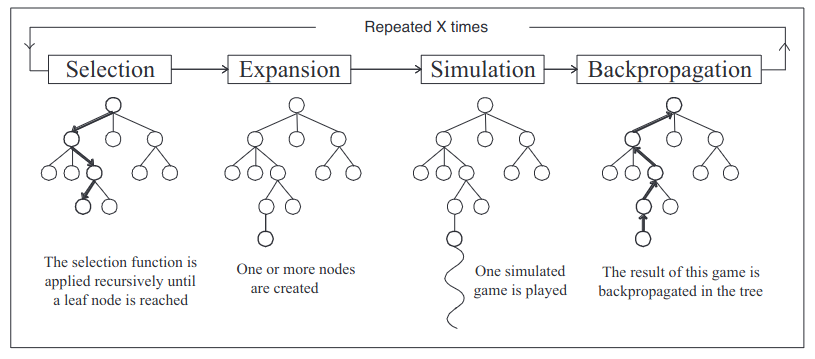
\includegraphics[width=\linewidth]{figures/mcts.png}
    \caption{MCTS example for a two player game such as chess.}
    \label{fig:mcts}
\end{figure}
